\documentclass[utf8]{beamer}
\usepackage [utf8]{inputenc}
\usepackage[russian]{babel}
\usepackage{caption}
\usepackage{cmap}
\usepackage[backend=bibtex]{biblatex}
\bibliography{DipBib}
\usepackage[T2A]{fontenc}
\usepackage{cmap}
\newsavebox{\longestsec}
\usetheme{Madrid}
\useoutertheme{tree}
\usepackage{epstopdf}
\usepackage{float}

\DeclareCaptionLabelFormat{andtable}{#1~#2  \&  \tablename~\thetable}


\renewcommand{\figurename}{Fig.}

\DeclareGraphicsExtensions{.eps} 

\newtheorem{mdefinition}{Определение}[section]
\newtheorem{mremark}{Примечание}[subsection]
\newtheorem{msuggest}{Предложение}[subsection]
\newtheorem{mclaim}{Утверждение}[subsection]
\newtheorem{mlemma}{Лемма}[subsection]
\newtheorem{mtheorem}{Теорема}
\newtheorem{mconseq}{Следствие}

\DeclareMathOperator{\argmax}{argmax}
\DeclareMathOperator{\argmin}{argmin}
\DeclareMathOperator{\grad}{grad}
\DeclareMathOperator{\sign}{sign}
\DeclareMathOperator{\diag}{diag}
\DeclareMathOperator{\norm}{norm}
\renewcommand{\leq}{\leqslant}
\renewcommand{\geq}{\geqslant}
\renewcommand{\phi}{\varphi}
\setcounter{figure}{0}


\title{Эксперименты по единственности разложения}
\date{17 мая 2017}


\begin{document}
	\begin{frame}
		\titlepage
	\end{frame}

	\begin{frame}
		\frametitle{Краткое содержание}
		\renewcommand{\baselinestretch}{1.5}
		\fontsize{12pt}{9.2}\selectfont
		\tableofcontents
	\end{frame}
	
\section{Зависимость от коэффициента разреживания}
	\begin{frame}	
	\frametitle{Зависимость от коэффициента разреживания. Описание эксперимента}
	\begin{enumerate}
\item Используем лемматизированный 20newsgroups.
\item Обучаем модель c с регуляризаторам $\alpha \sum_{w, t} \log \phi_{wt} + \beta \sum_{t, d} \log \theta_{td}$ при разных $\alpha$ и $\beta$ и считаем  среднюю меру единственности по темам.
\end{enumerate}
	\end{frame}
	\begin{frame}	
	\begin{figure}[h]
	\frametitle{Зависимость от коэффициента разреживания}
	\centering  	
	\caption{20newsgroup 3 метки. В разложении $|T| = 5$} 
	\medskip
	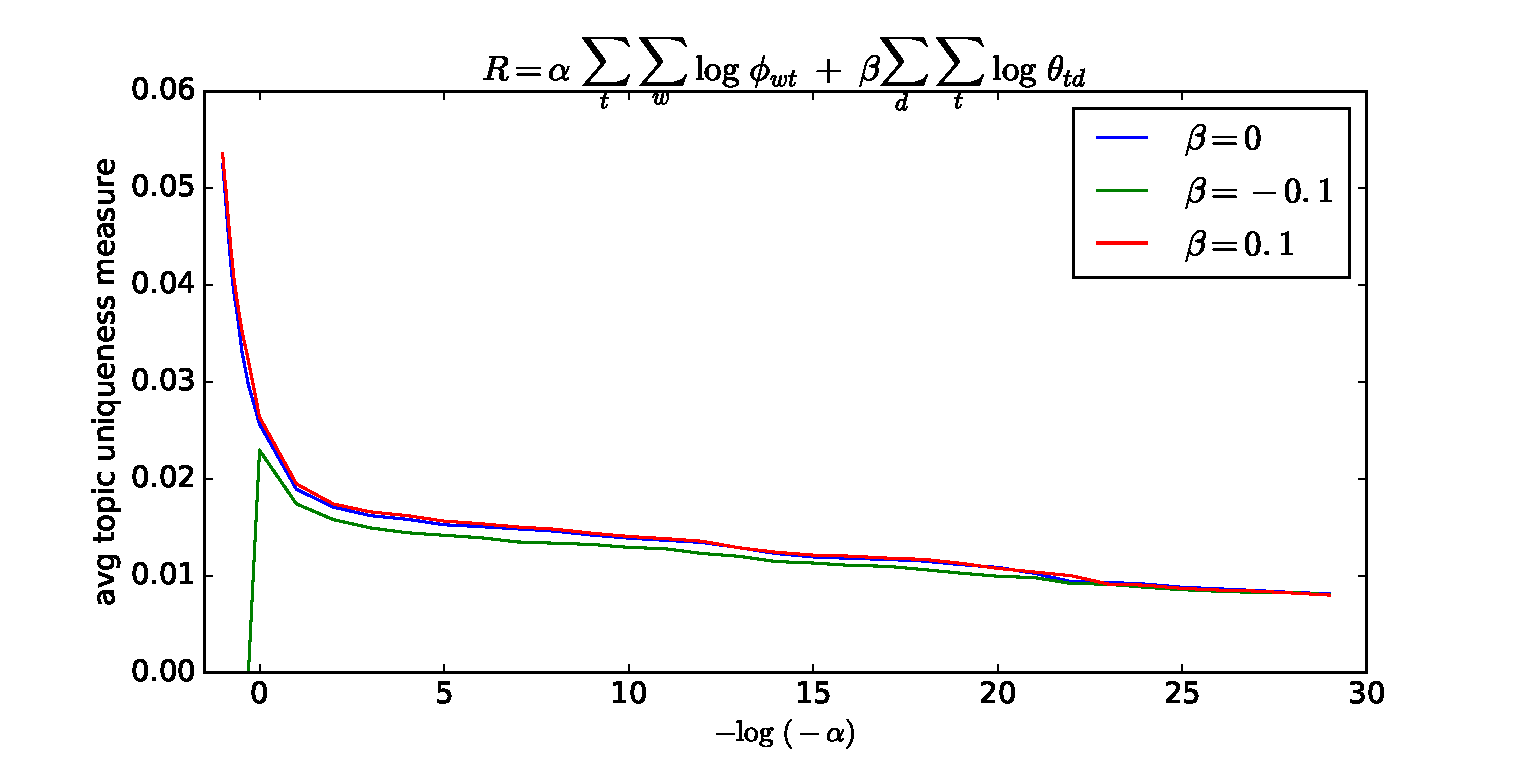
\includegraphics[width=0.9\linewidth]{presentation_pictures/alpha_dependency_topics_origin_3_ums.eps}  
	\end{figure}
	\end{frame}
	
	\begin{frame}	
	\begin{figure}[h]
	\frametitle{Зависимость от коэффициента разреживания}
	\centering  	
	\caption{20newsgroup 7 меток. В разложении $|T| = 10$} 
	\medskip
	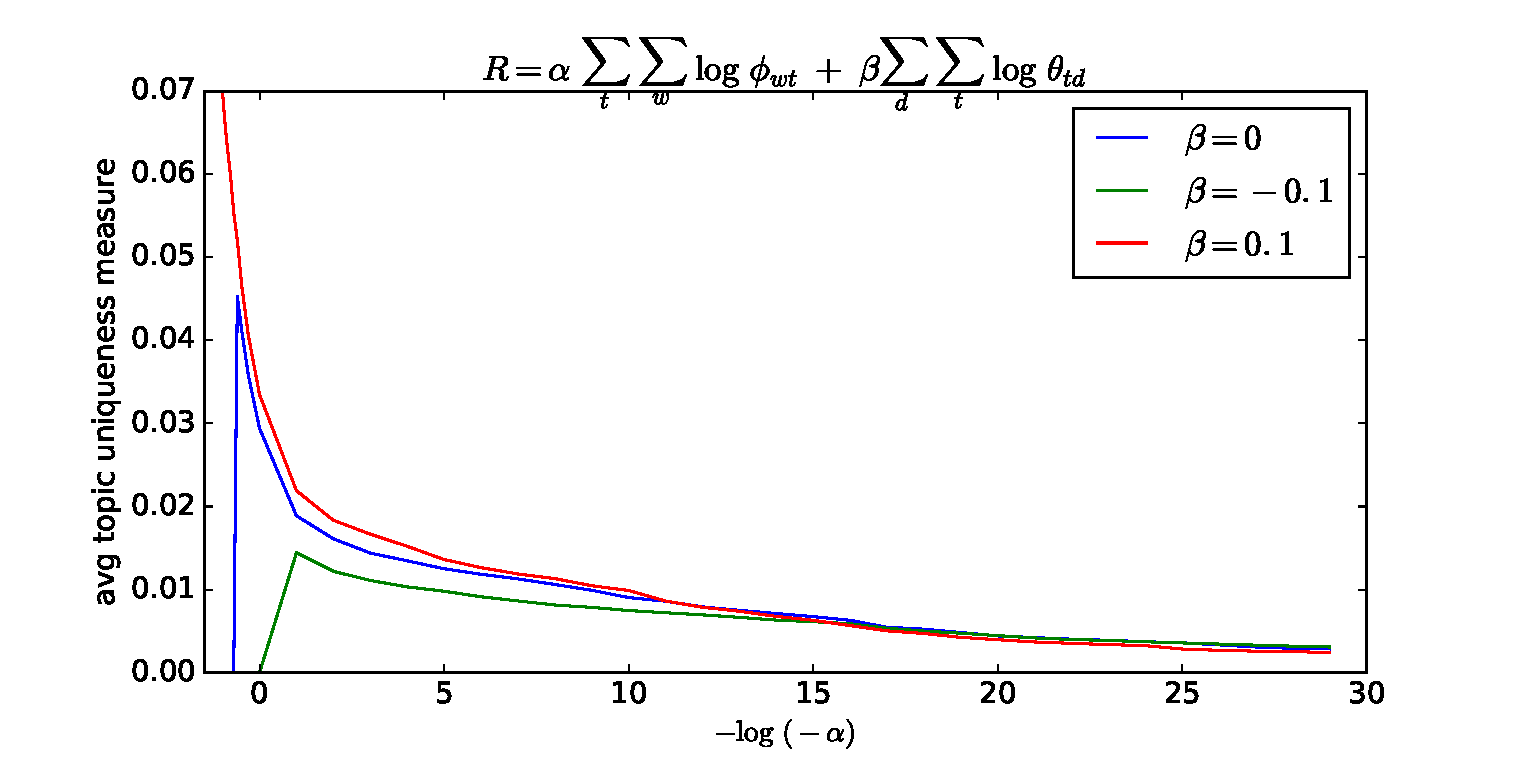
\includegraphics[width=0.9\linewidth]{presentation_pictures/alpha_dependency_topics_origin_7_ums.eps}  
	\end{figure}
	\end{frame}
	
	\section{Зависимость от числа тем}
	\begin{frame}	
	\frametitle{Зависимость от числа тем. Описание эксперимента}
	\begin{enumerate}
\item Используем лемматизированный 20newsgroups с разным числом меток.
\item 10 процентов слов в каждом документе скрываем.
\item Обучаем модель на трейне и считаем меру единственности для каждой темы. Отслеживаем минимальное (по темам), максимальное и среднее.
\item У получившейся модели считаем перплексию на тесте.
\end{enumerate}
	\end{frame}
	
	\begin{frame}	
	\frametitle{Зависимость от числа тем. 1 метка}
	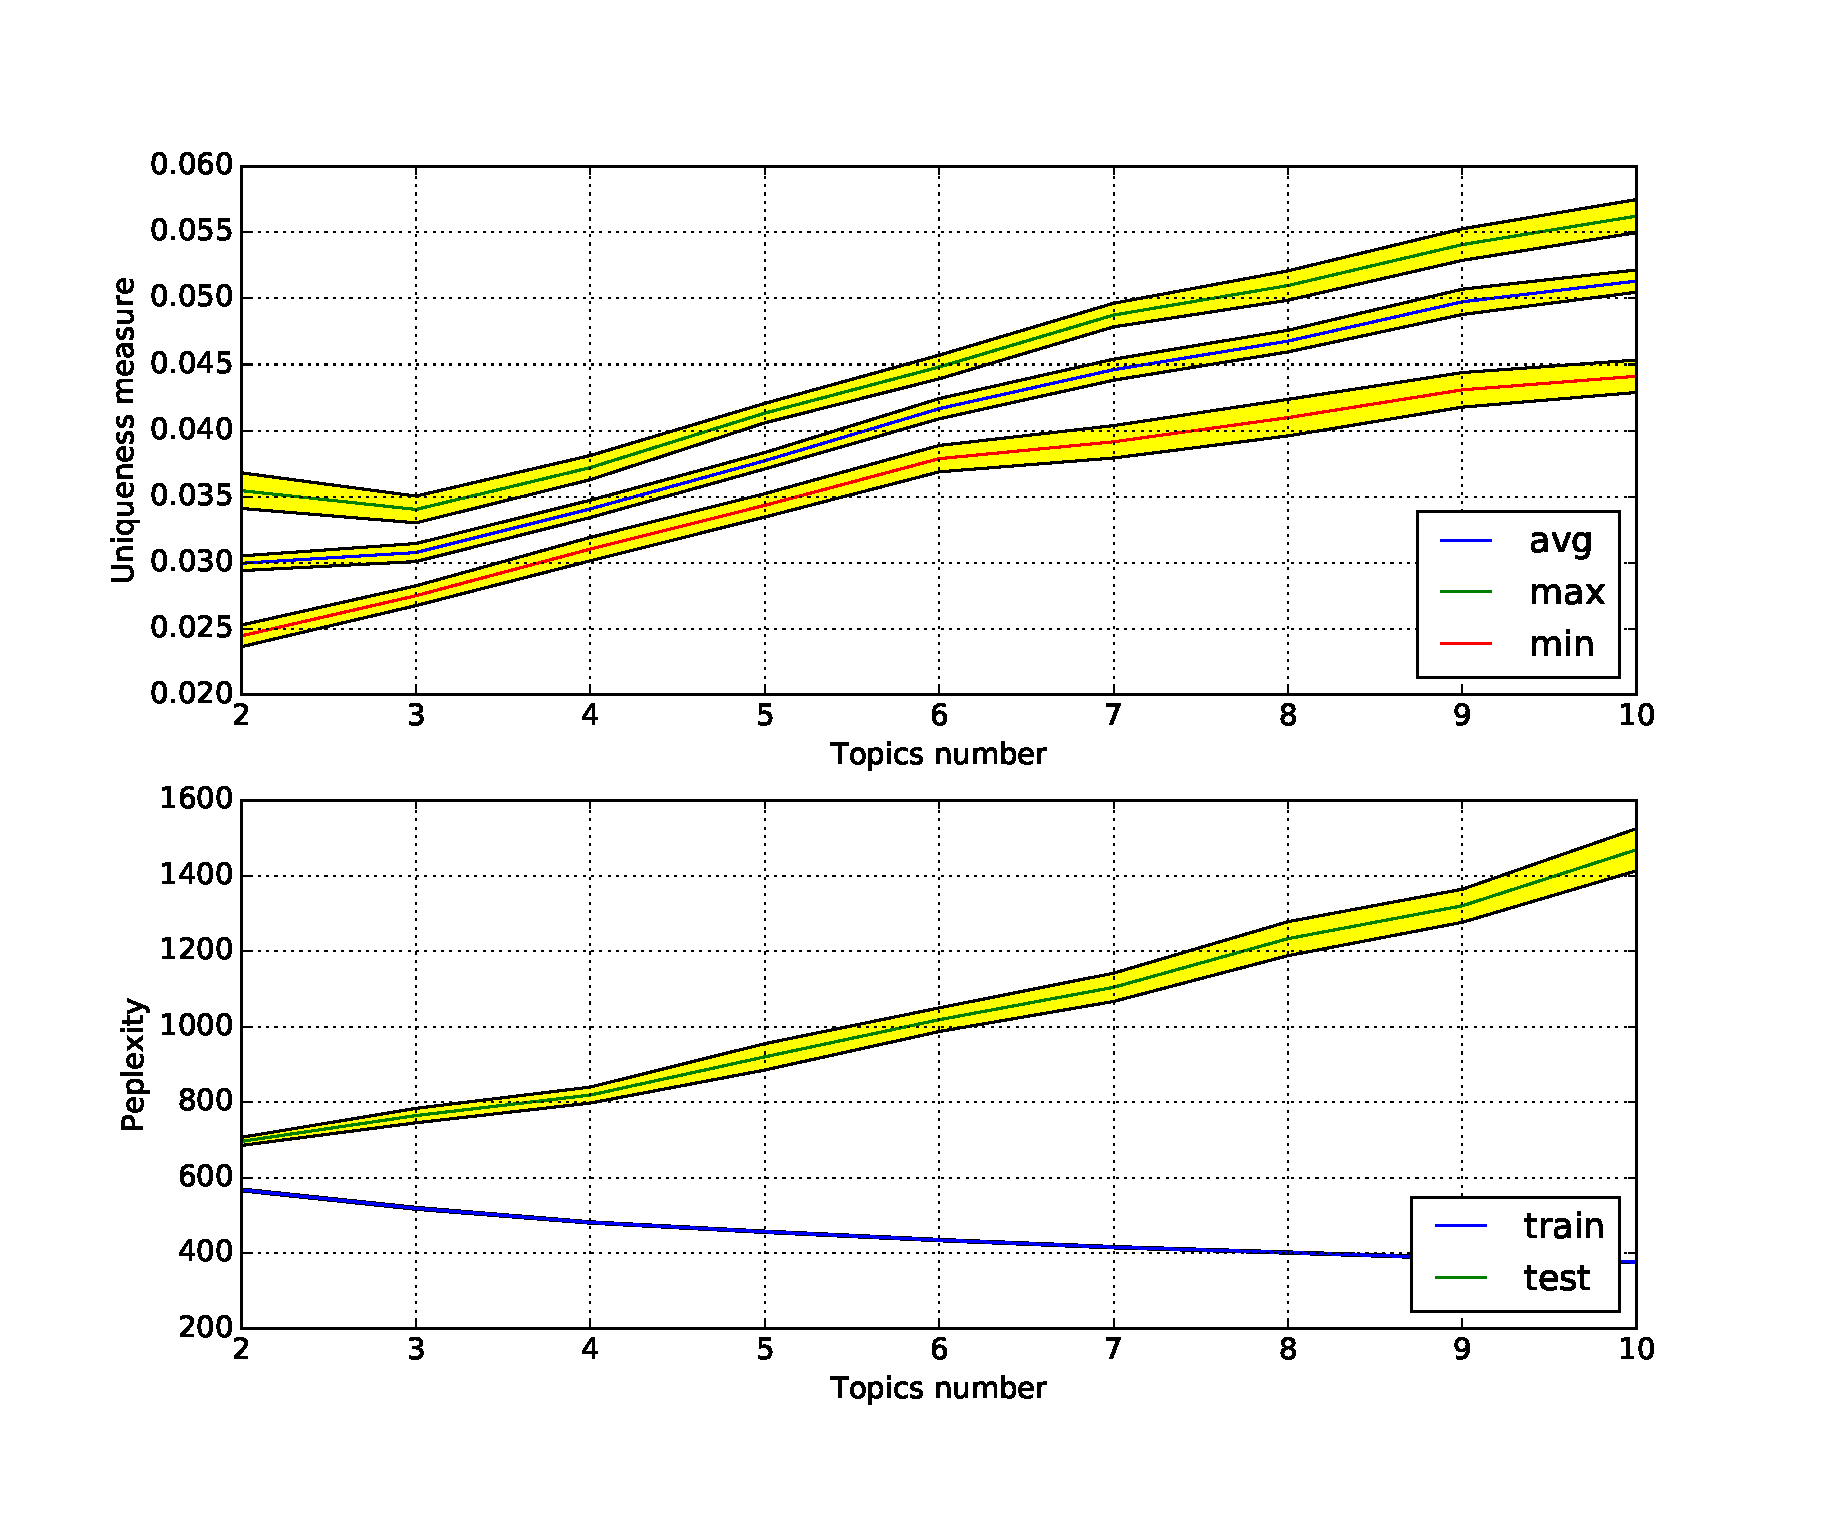
\includegraphics[width=0.75\linewidth]{presentation_pictures/topics_dependency_origin_1_ums.eps} 
	\end{frame}
	
	\begin{frame}	
	\frametitle{Зависимость от числа тем. 2 метки}
	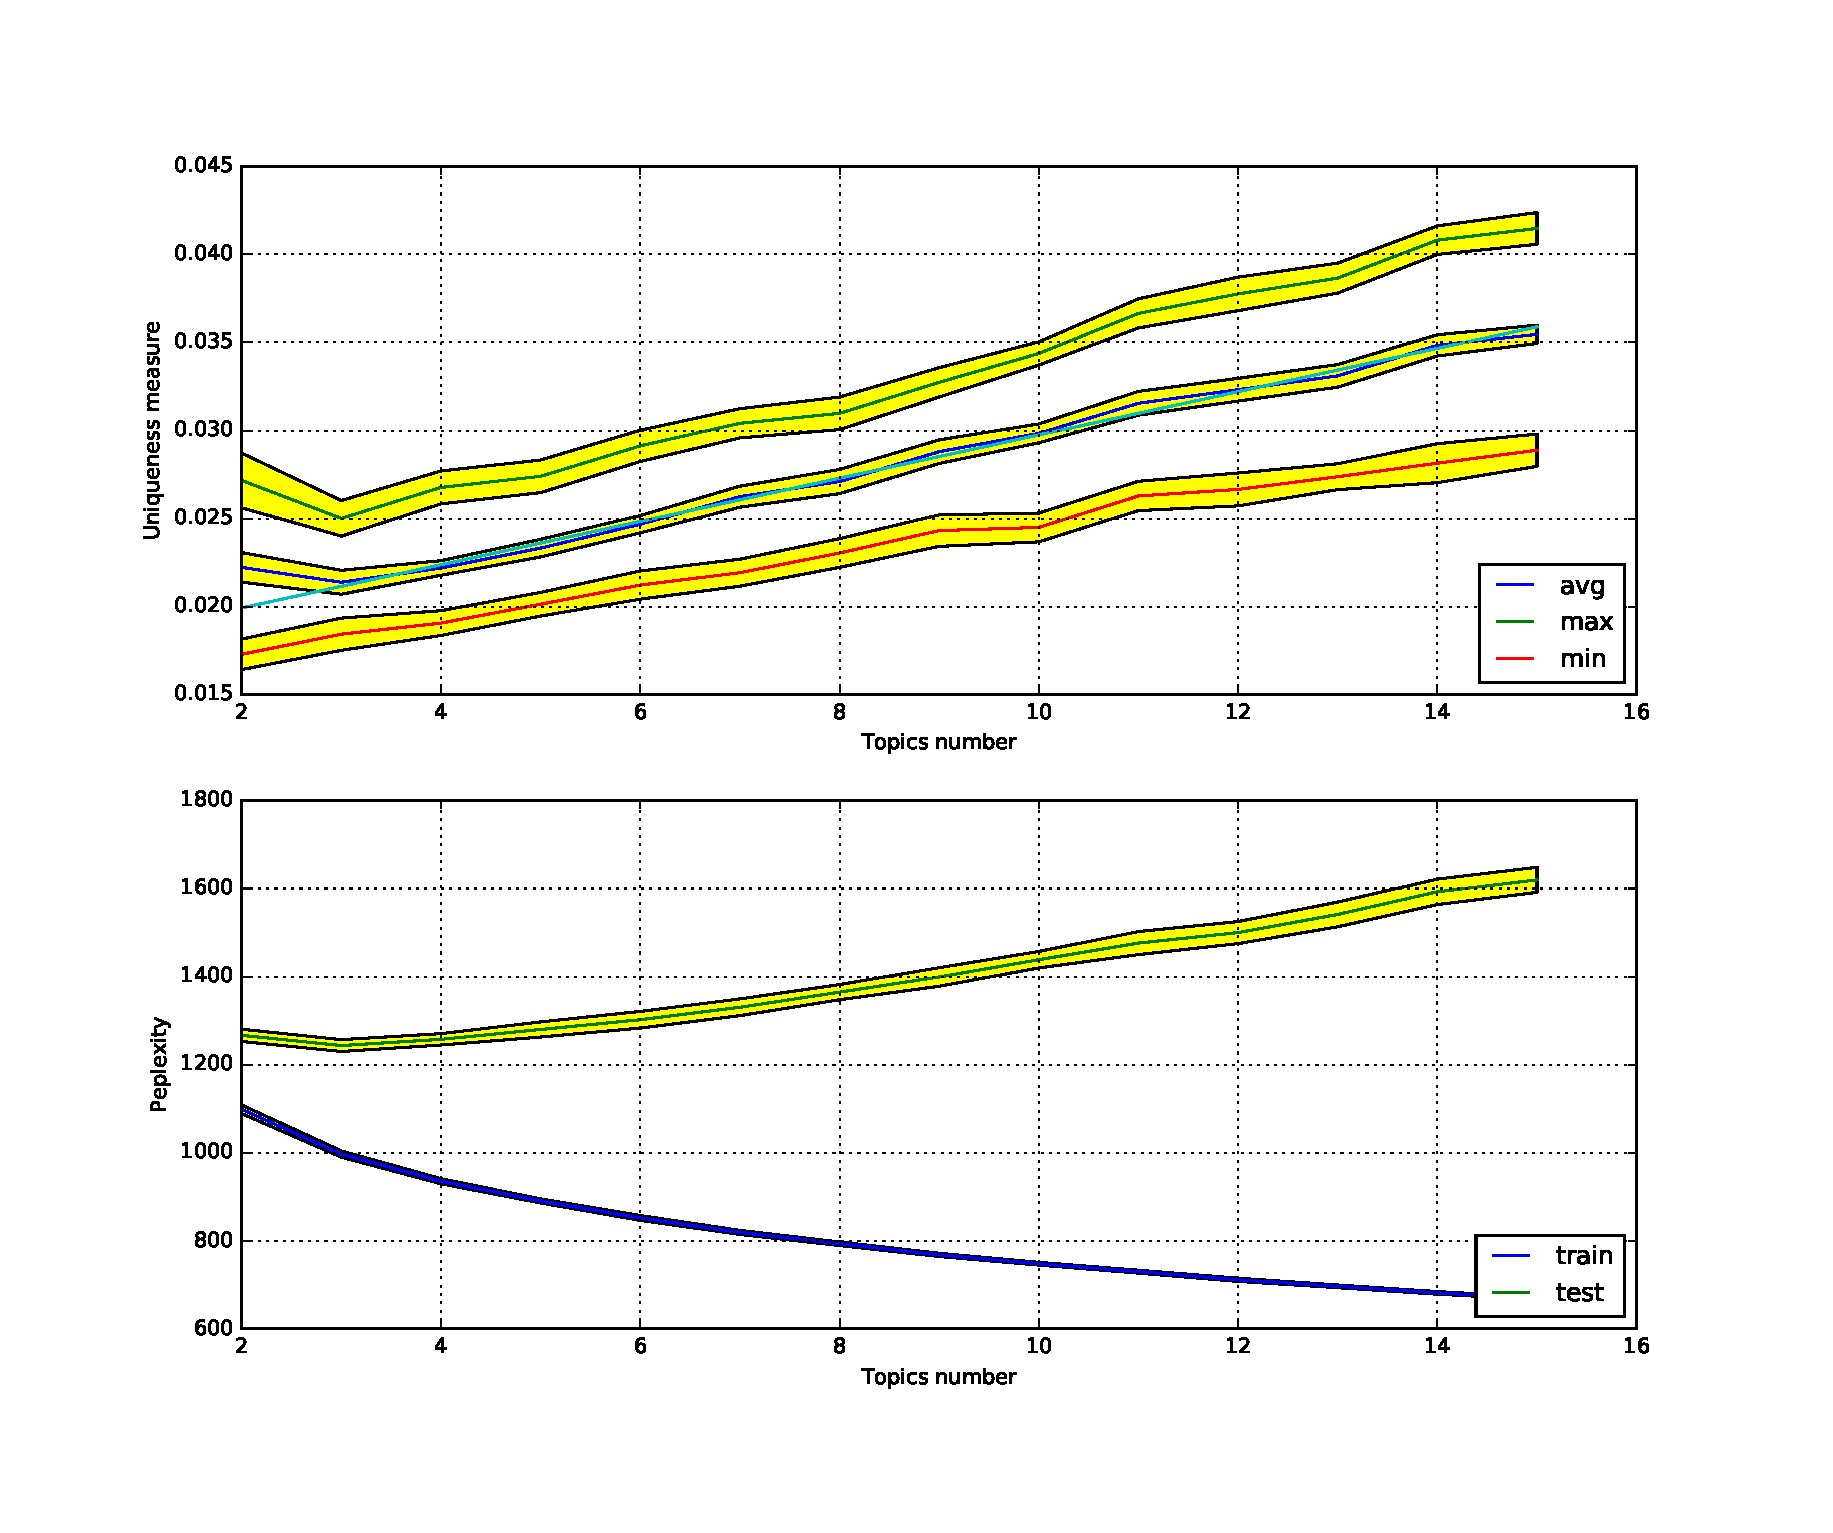
\includegraphics[width=0.75\linewidth]{presentation_pictures/topics_dependency_origin_2_ums.eps} 
	\end{frame}
	
	\begin{frame}	
	\frametitle{Зависимость от числа тем. 3 метки}
	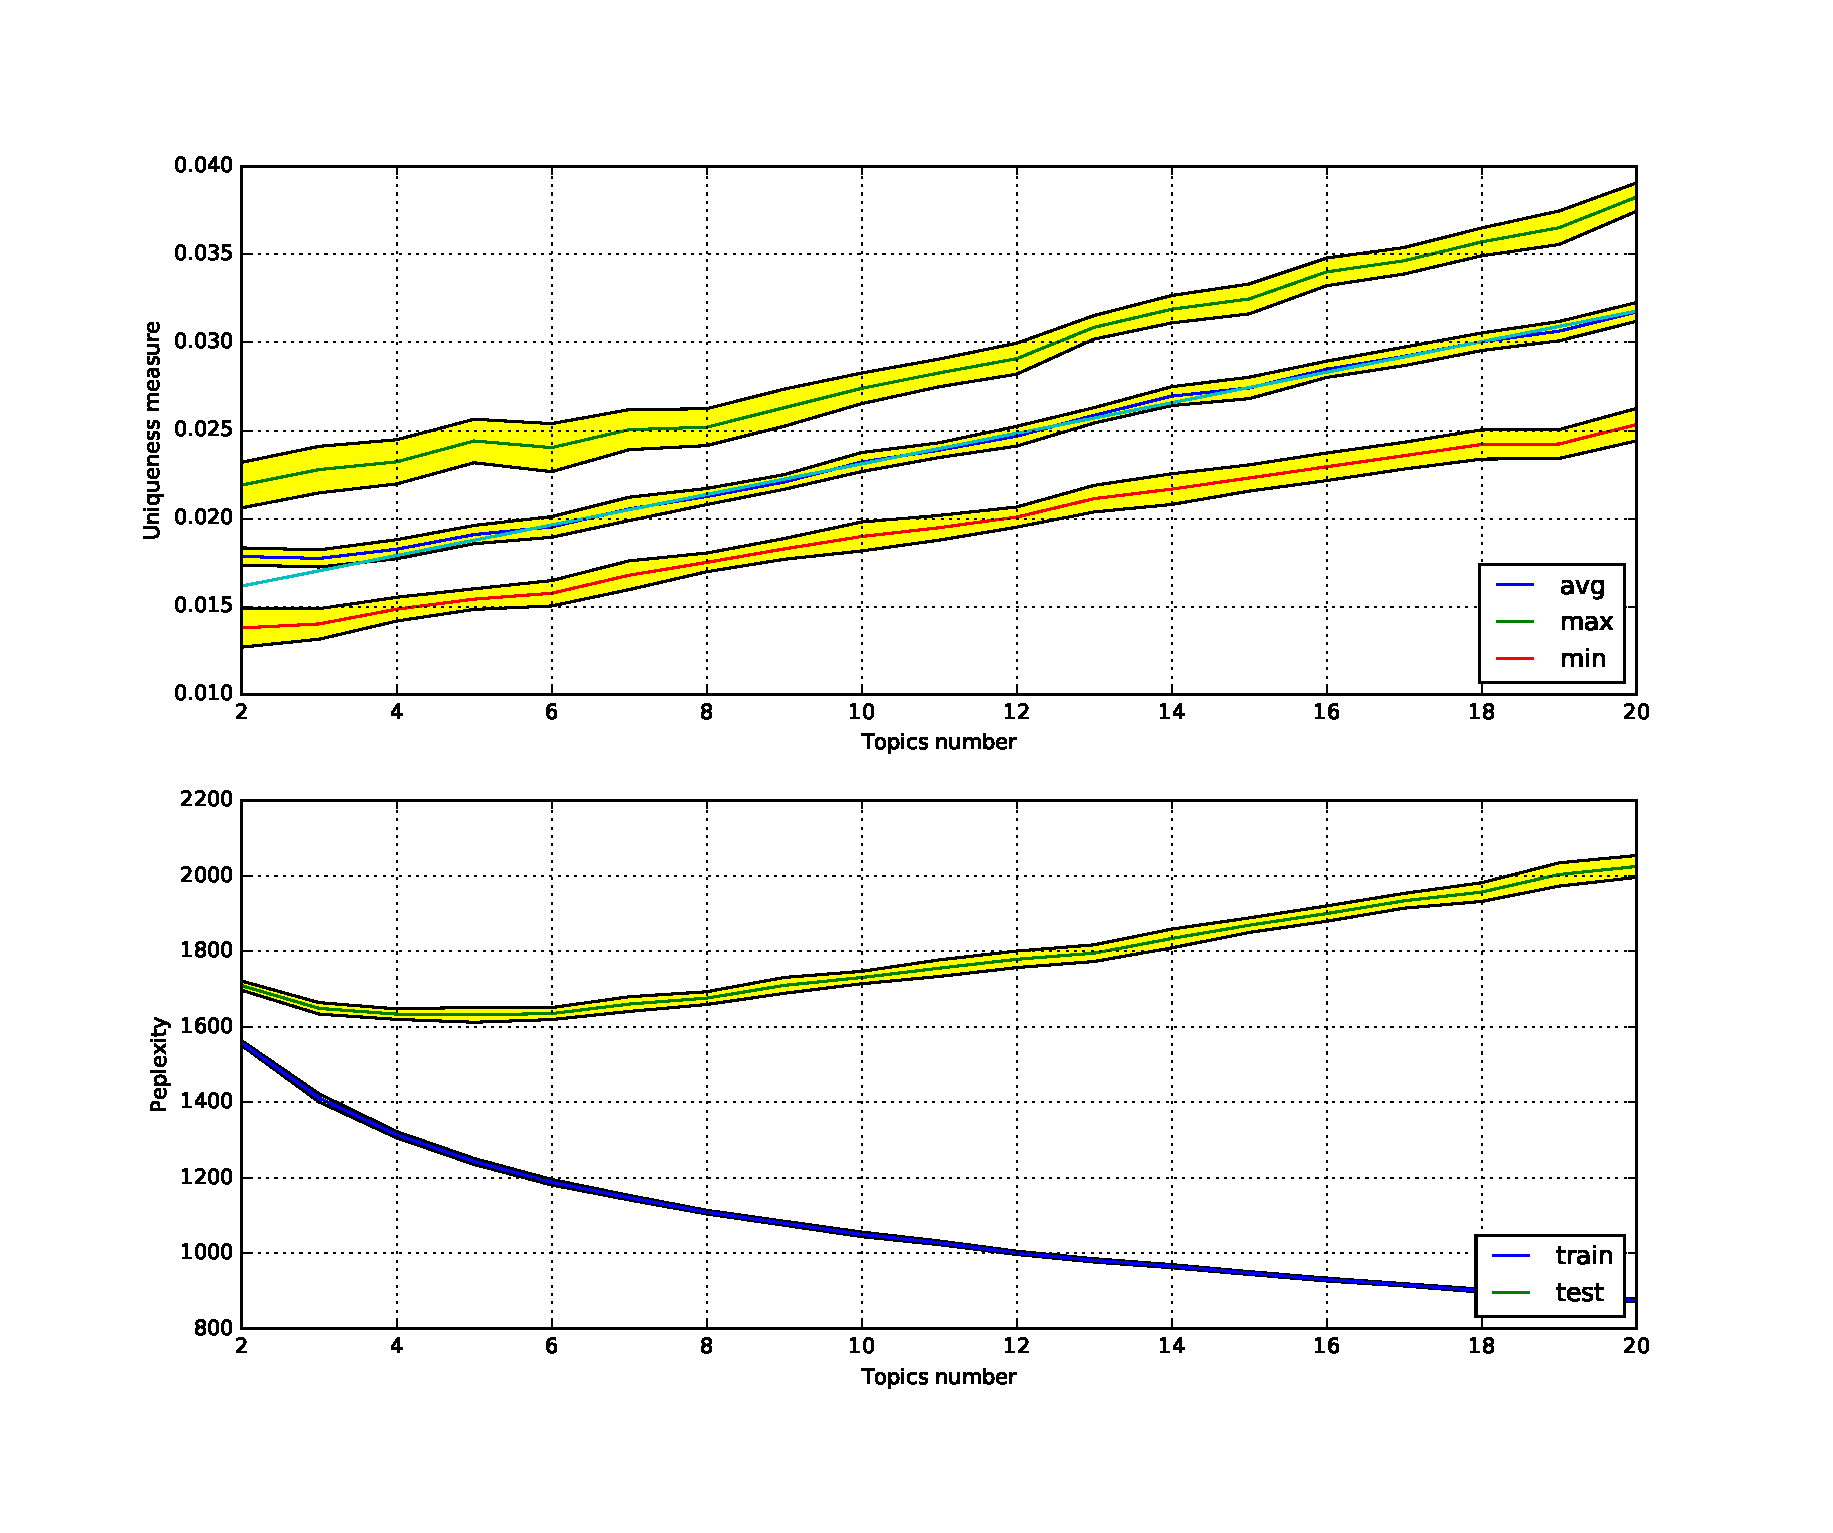
\includegraphics[width=0.75\linewidth]{presentation_pictures/topics_dependency_origin_3_ums.eps} 
	\end{frame}
	
	
	\begin{frame}	
	\frametitle{Зависимость от числа тем. 3 метки}
	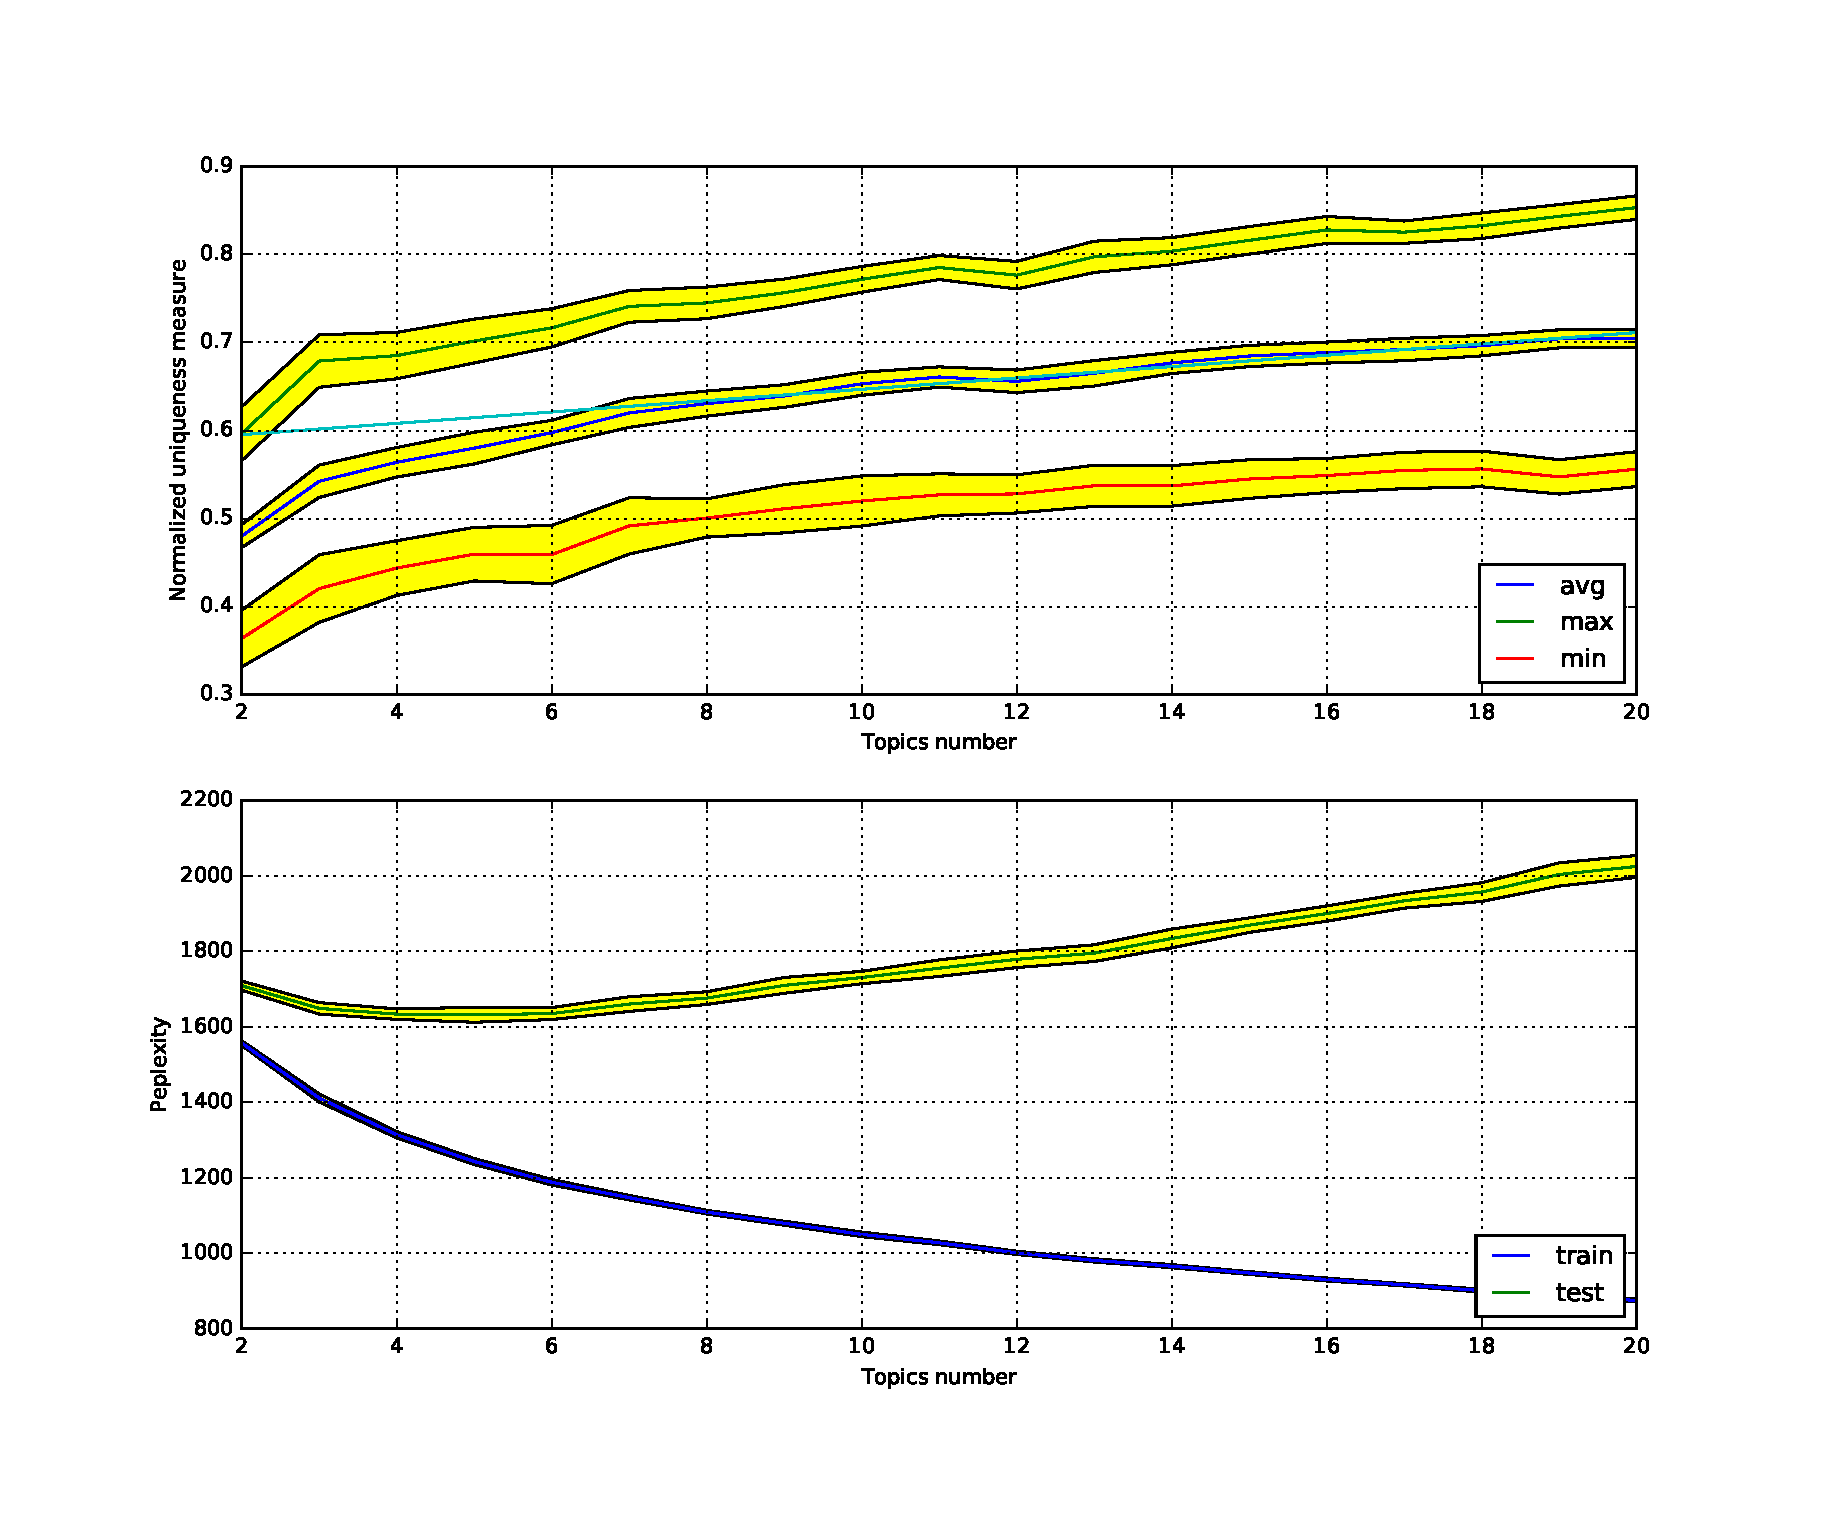
\includegraphics[width=0.75\linewidth]{presentation_pictures/topics_dependency_origin_3_nums.eps} 
	\end{frame}
	
	
	\begin{frame}	
	\frametitle{Зависимость от числа тем. 4 метки}
	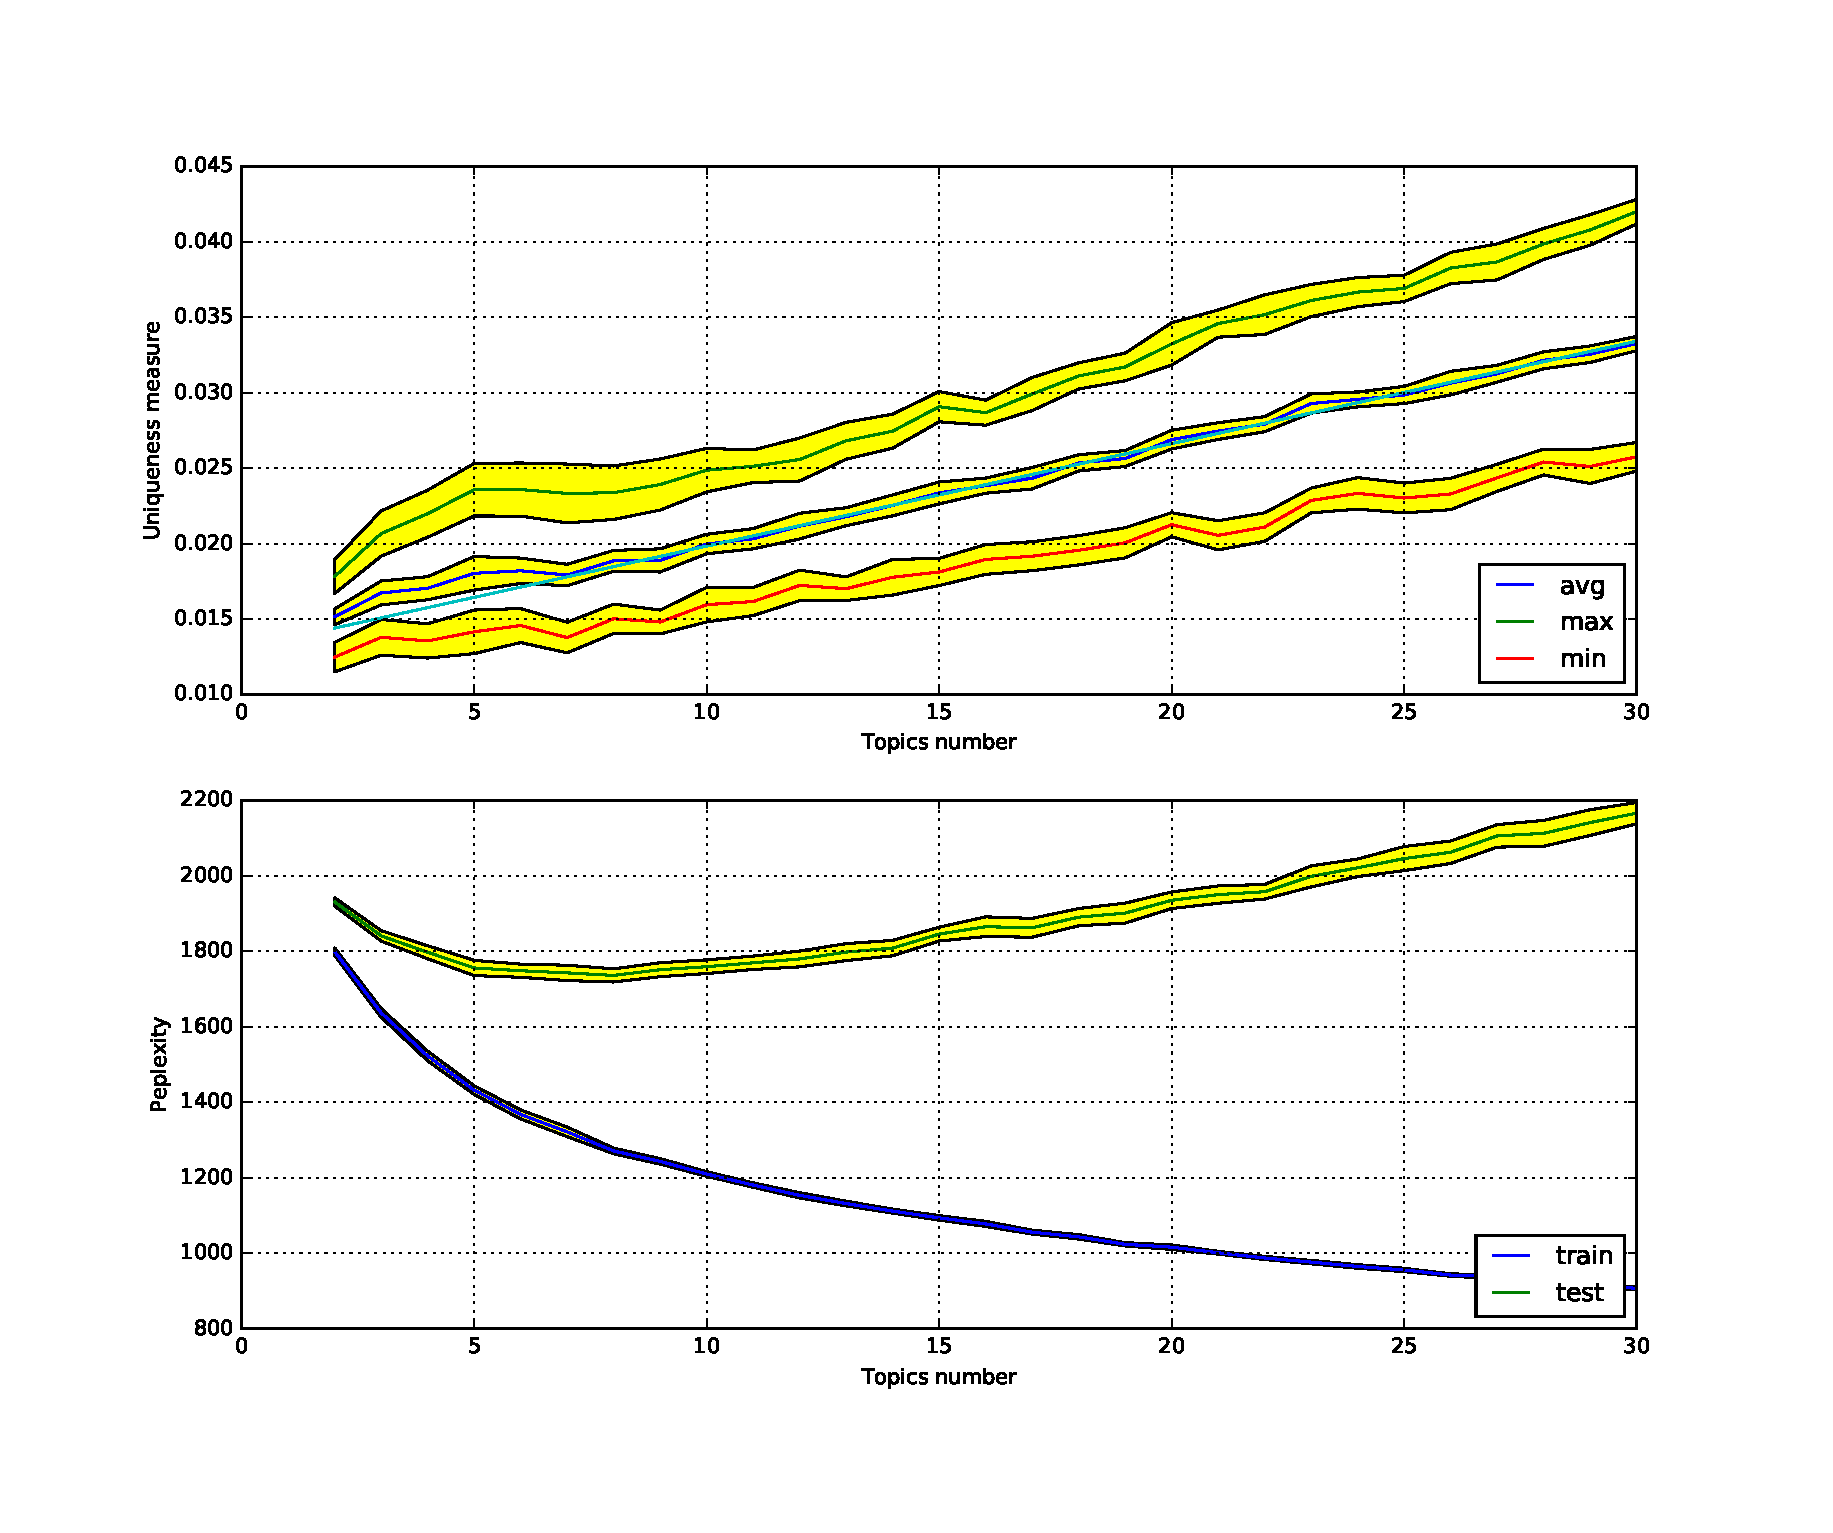
\includegraphics[width=0.75\linewidth]{presentation_pictures/topics_dependency_origin_4_ums.eps} 
	\end{frame}

	
	\begin{frame}	
	\frametitle{Зависимость от числа тем. 7 меток}
	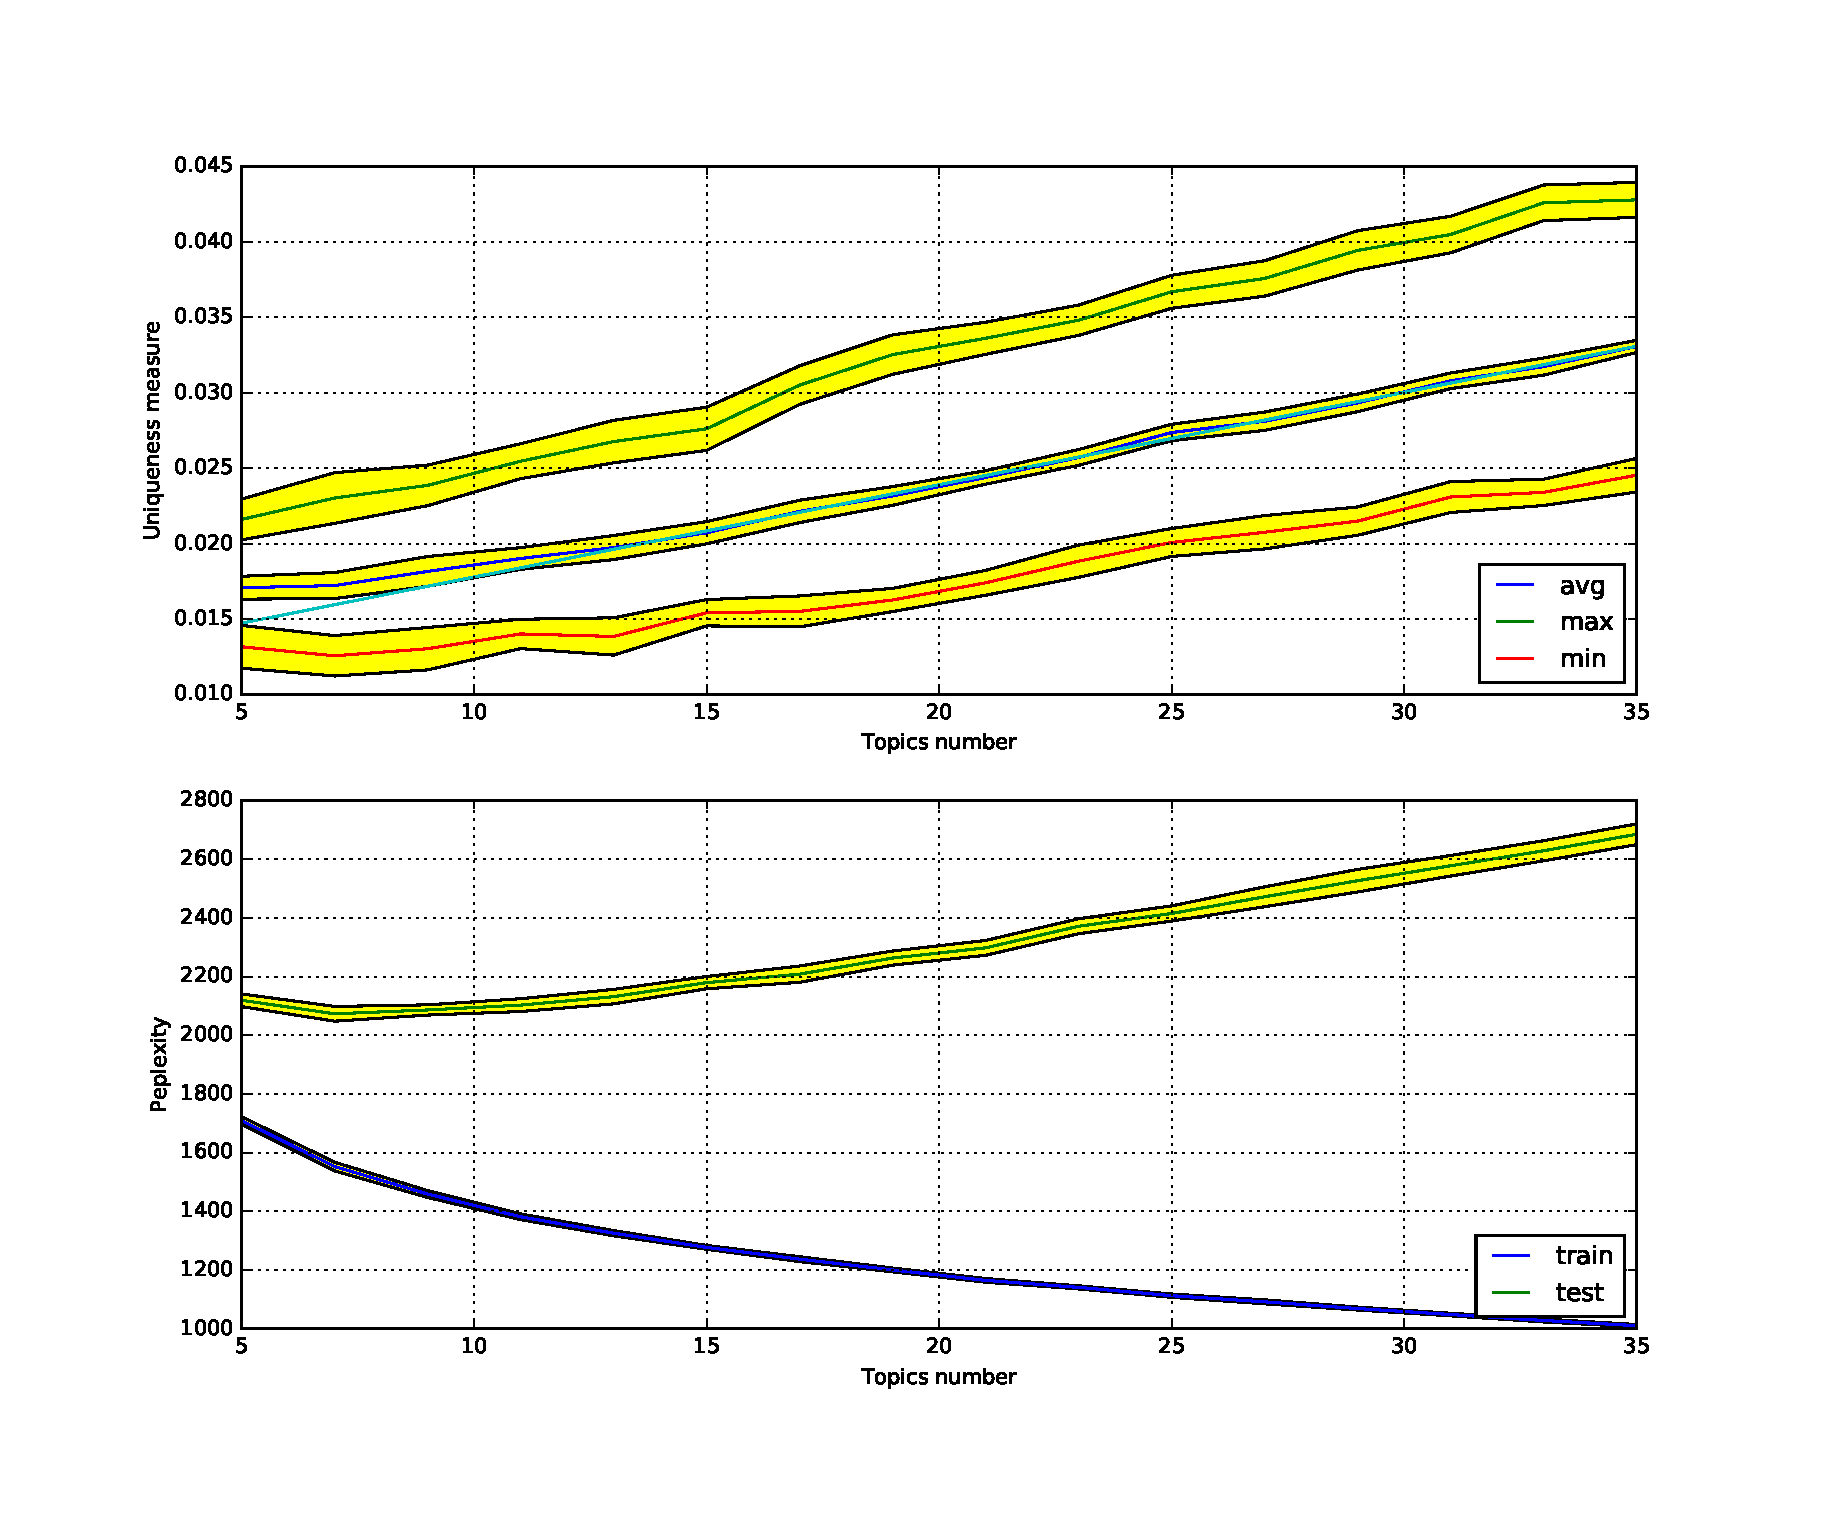
\includegraphics[width=0.75\linewidth]{presentation_pictures/topics_dependency_origin_big_ums.eps} 
	\end{frame}
	
	\section{Проверка уникальности}
	\begin{frame}	
	\frametitle{Проверка уникальности. Описание эксперимента}
	\begin{enumerate}
\item Используем лемматизированный 20newsgroups с 3 метками (sci.med, sci.electronics, sci.space).
\item Обучаем разреженную модель и по ней получаем синтетическую матрицу документ-слова. 
\item Исследуем разброс и смещение разных метрик в зависимости от начальной инициализации и природы данных.
\end{enumerate}
	\end{frame}
	
	\begin{frame}	
	\frametitle{Проверка уникальности. Обозначения метрик}
	\begin{enumerate}
\item L1(p, q). $\sum_k |p_k - q_k|$
\item sMAPE(p, q). $\frac1n \sum_k \frac{|p_k - q_k|}{|p_k| + |q_k|}$
\item KL(p, q). $\sum_k p_k \frac{p_k}{q_k}$
\item KL2(p, q). $KL(p, z) + KL(q, z)$, где $z = \frac{p + q}{2}$
\item Обучаем разреженную модель и по ней получаем синтетическую матрицу документ-слова. 
\item Исследуем разброс и смещение разных метрик в зависимости от начальной инициализации и природы данных.
\end{enumerate}
	\end{frame}
	
	\begin{frame}	
	\fontsize{10pt}{9.2}\selectfont
	\frametitle{Проверка уникальности. PLSA}
	 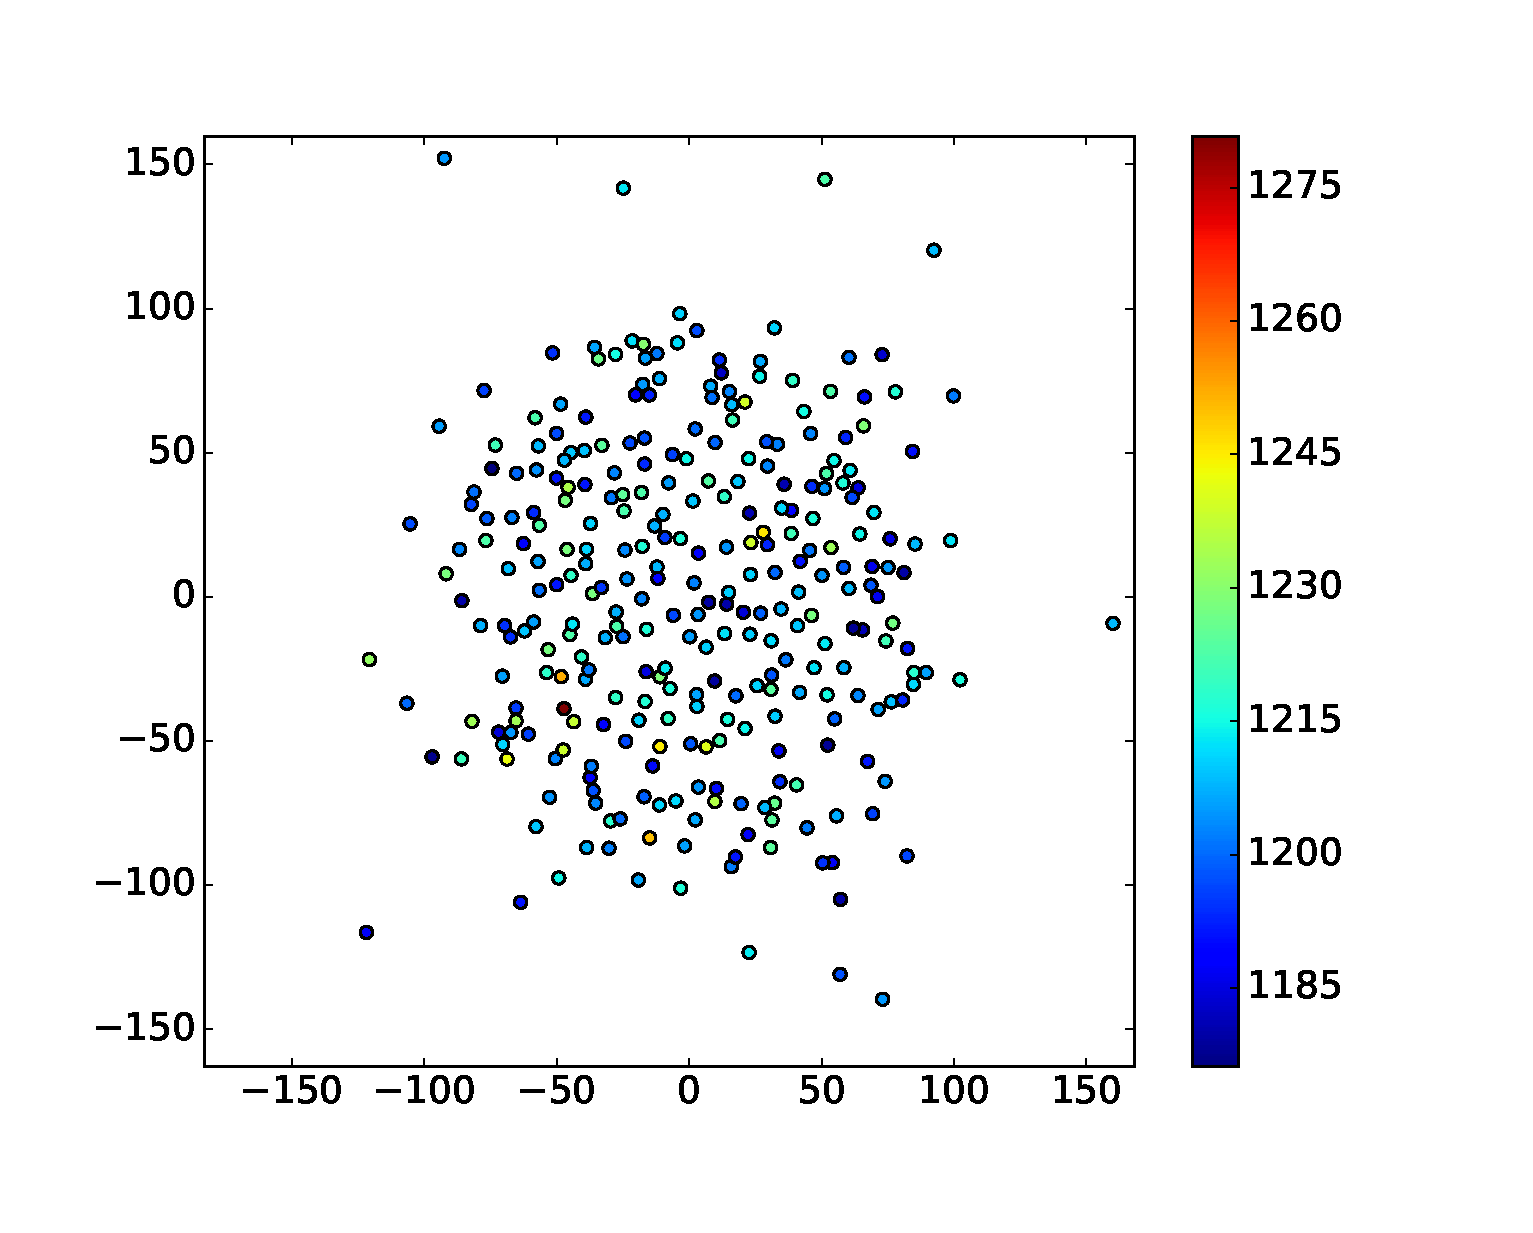
\includegraphics[width=0.45\linewidth]{presentation_pictures/plsa.eps} 
    \begin{tabular}[b]{| l | l | }\hline
      Variance L1 & $0.5767 \pm 0.0028$ \\ \hline
      Variance sMAPE  & $1.1187 \pm  0.0026$ \\ \hline
      Variance KL  & $2.9310 \pm 0.0301$ \\ \hline
      Variance KL2  & $0.2147 \pm 0.0015$ \\ \hline

      Bias L1 & None \\ \hline
      Bias sMAPE  & None \\ \hline
      Bias KL  & None \\ \hline
      Bias KL2  & None \\ \hline
    \end{tabular}

	\end{frame}
	
	
	\begin{frame}	
	\fontsize{10pt}{9.2}\selectfont
	\frametitle{Проверка уникальности. Initialized PLSA}
	 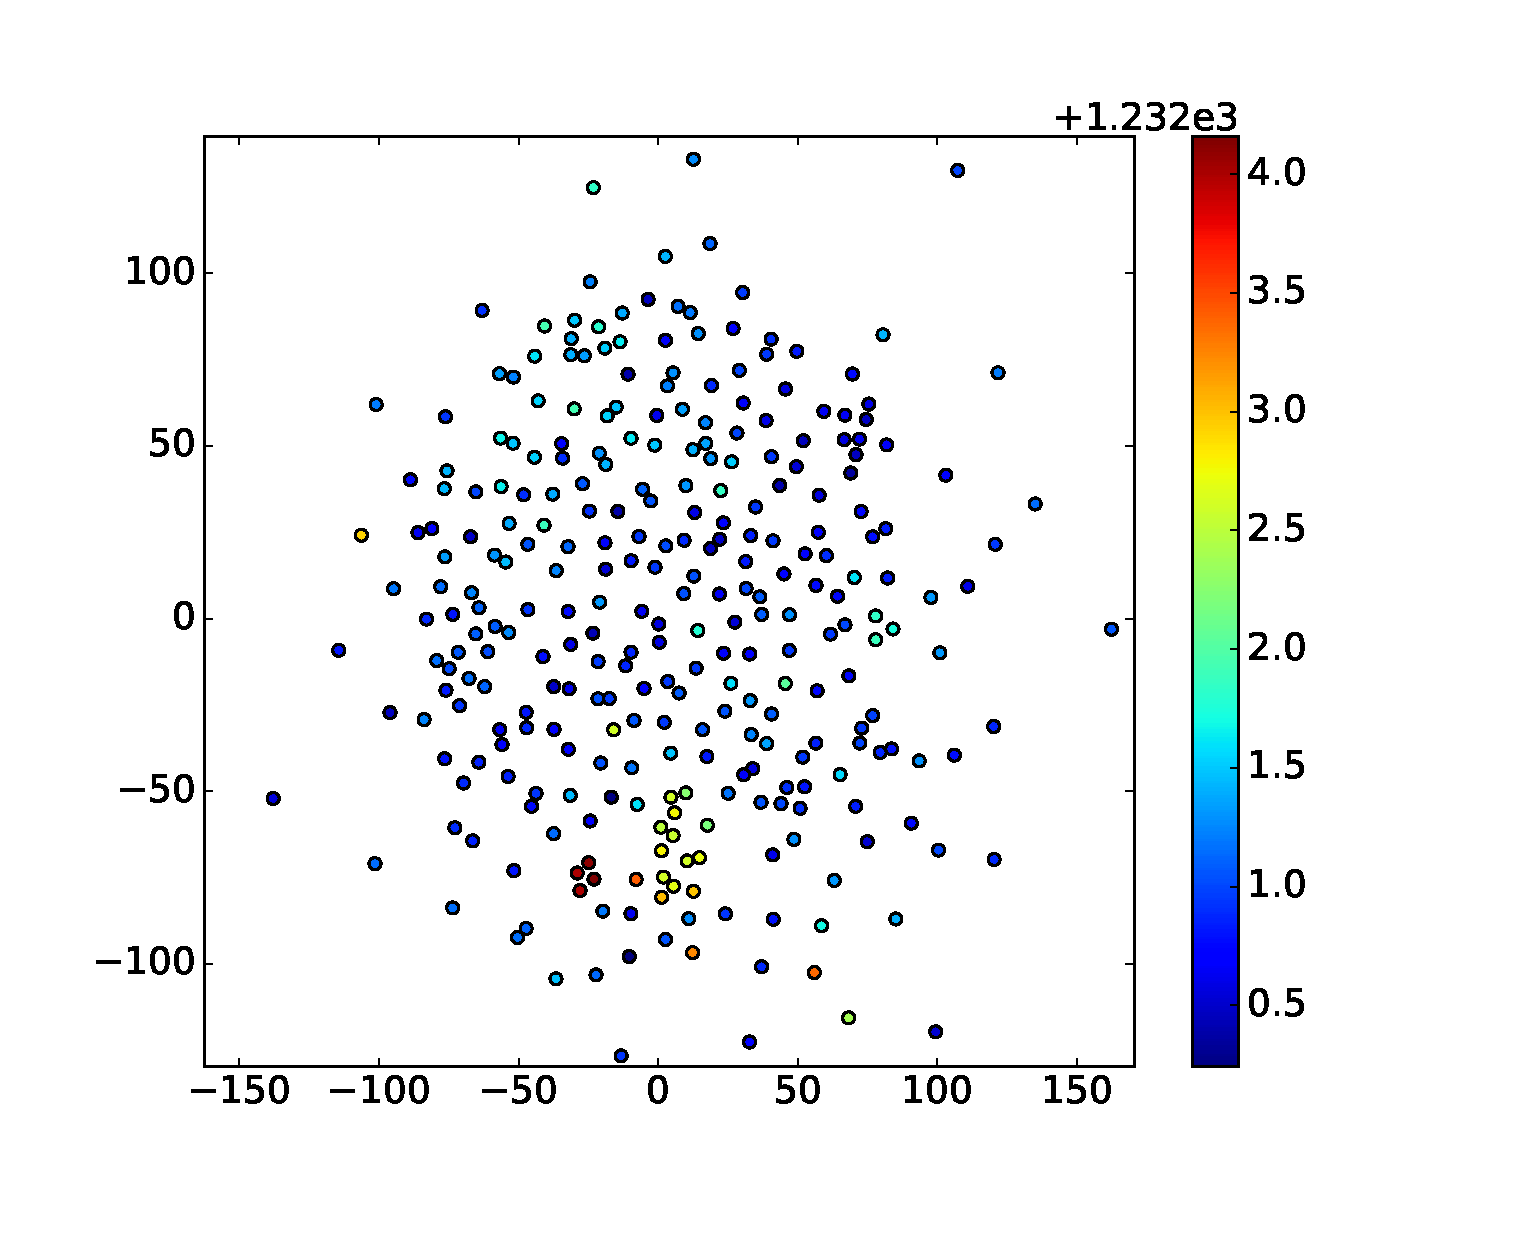
\includegraphics[width=0.45\linewidth]{presentation_pictures/full_initialized_plsa.eps} 
    \begin{tabular}[b]{| l | l | }\hline
      Variance L1 & $0.0529 \pm 0.0006$ \\ \hline
      Variance sMAPE  & $0.1199 \pm 0.0008$ \\ \hline
      Variance KL  & $0.0189 \pm 0.0006 $ \\ \hline
      Variance KL2  & $0.0052 \pm 0.0001$ \\ \hline

      Bias L1 & $0.0421 \pm 0.0061$ \\ \hline
      Bias sMAPE  & $0.1004 \pm 0.0058$ \\ \hline
      Bias KL  & $0.0163 \pm 0.0079$ \\ \hline
      Bias KL2  & $0.0036 \pm 0.0012$ \\ \hline
    \end{tabular}

	\end{frame}
	
	
	\begin{frame}
	\fontsize{10pt}{9.2}\selectfont
	\frametitle{Проверка уникальности. Syntetic PLSA}
	 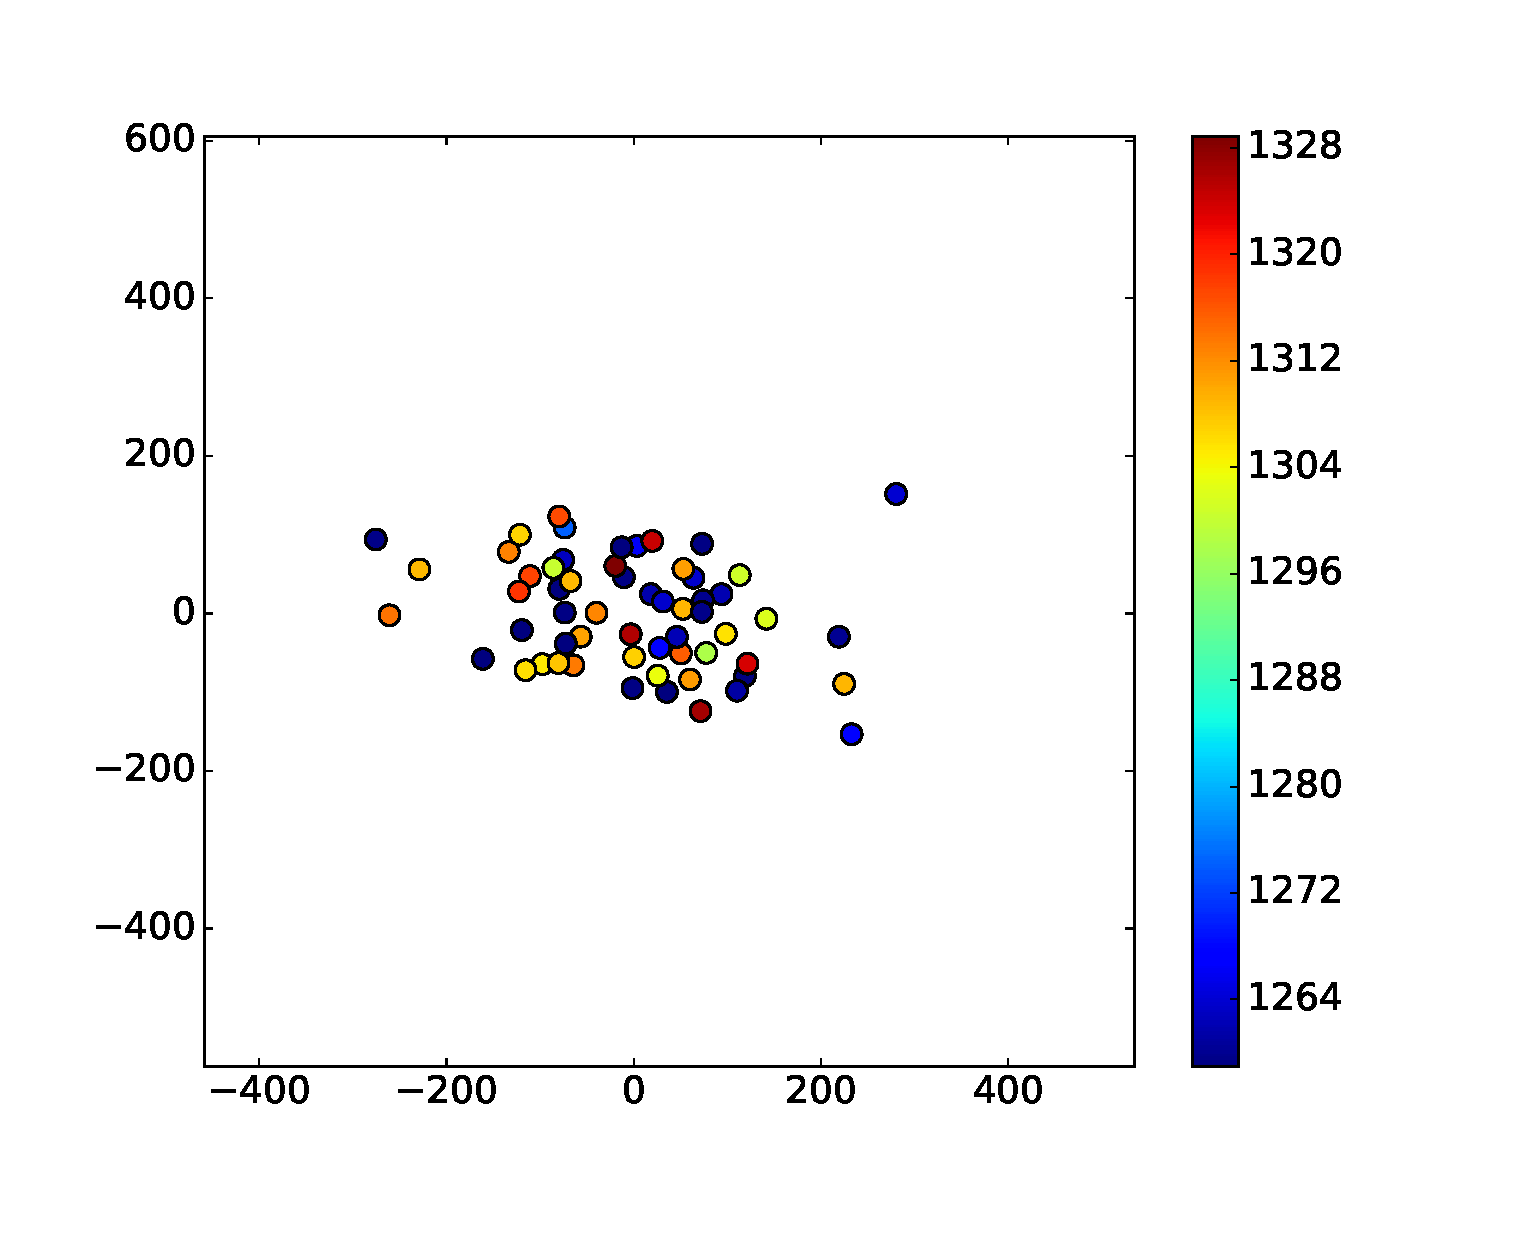
\includegraphics[width=0.45\linewidth]{presentation_pictures/syntetic_plsa.eps} 
    \begin{tabular}[b]{| l | l | }\hline
      Variance MAE & $0.2780 \pm 0.0198$ \\ \hline
      Variance sMAPE  & $0.9471 \pm 0.0159$ \\ \hline
      Variance KL  & $0.2491 \pm 0.0287$ \\ \hline
      Variance KL2  & $0.0758 \pm 0.0075$ \\ \hline

      Bias MAE & $0.2197 \pm 0.1199$ \\ \hline
      Bias sMAPE  & $1.0700 \pm 0.0637$ \\ \hline
      Bias KL  & $0.1343 \pm 0.0969$ \\ \hline
      Bias KL2  & $0.0696 \pm 0.0496$ \\ \hline
    \end{tabular}

	\end{frame}
	
	
	\begin{frame}	
	\fontsize{10pt}{9.2}\selectfont
	\frametitle{Проверка уникальности. Initialized Syntetic PLSA}
	 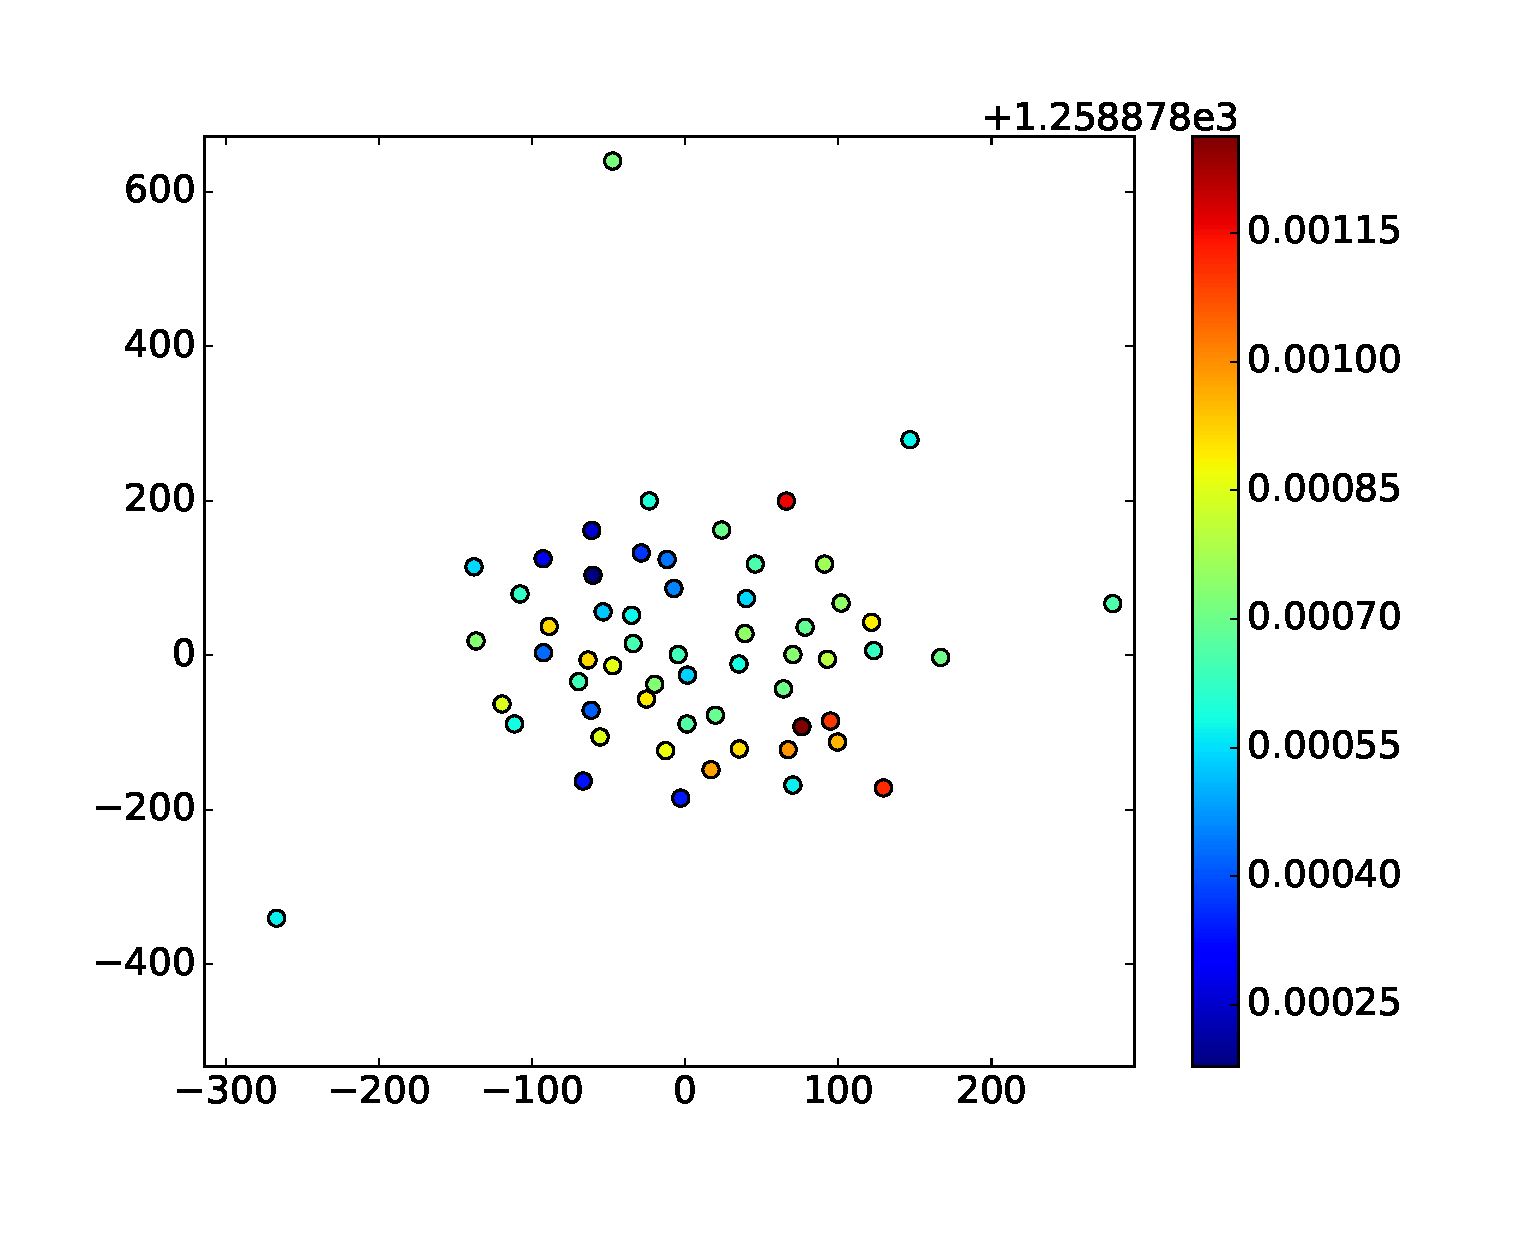
\includegraphics[width=0.45\linewidth]{presentation_pictures/full_initialized_syntetic_plsa.eps} 
    \begin{tabular}[b]{| l | l | }\hline
      Variance MAE & $(6.8219 \pm 0.6114)  \cdot10^{-5}$ \\ \hline
      Variance sMAPE  & $0.0011 \pm 0.0001$ \\ \hline
      Variance KL  & $(8.9334 \pm 1.8492)  \cdot10^{-7}$ \\ \hline
      Variance KL2  & $(4.4434 \pm 0.9180)  \cdot10^{-7}$ \\ \hline

      Bias MAE & $0.0007 \pm 0.0001$ \\ \hline
      Bias sMAPE  & $0.0079 \pm 0.0023$ \\ \hline
      Bias KL  & $(6.6184 \pm 4.9818)  \cdot10^{-5}$ \\ \hline
      Bias KL2  & $(4.1158 \pm 3.1139)  \cdot10^{-5}$ \\ \hline
    \end{tabular}

	\end{frame}
	
	

\begin{frame}{Выводы}
\begin{enumerate}
\item Даже мизерного разреживания достаточно, чтобы обеспечить единственность разложения. Скорее нужно волноваться, что модель выродится, нежели станет неединственное разложение иметь.
\item Были введены две новых меры единственноости разложения. Они имеют явную связь с переобучением модели.
\item На реальных данных если фиксировать маску нулей в матрицах $\Phi$ и $\Theta$, разложение становится существенно устойчивее. Но не единственным!
\item На синтетических данных если фиксировать маску нулей в матрицах $\Phi$ и $\Theta$, разложение становится  почти единственное (колебания на уровне точности вычислений).
\end{enumerate}
\end{frame}

\end{document}
